\chapter{Methodology}
This chapter explores how GPUs convey information using a shared memory and defines what communication means in the context of this work. With this definition, the analysis space is described and explored.
\section{GPU Shared Memory Communication}
Other than the explicit communication routines of MPI like send and receive, GPUs convey information implicitly via the global memory on the device. 
The CUDA execution model and the given guarantees can be mapped to the Bulk-Synchronous-Parallel (BSP) bridging model, explained in \ref{bsp}.
\begin{itemize}
	\item \textbf{Computation} is a kernel executed on the GPU. The local processors in the model are represented by CTAs on a GPU, each processing it's own workload without the ability to directly
	interact with other CTAs.
	\item \textbf{Communication} in this step data generated in the computation step is placed in a location where it can be accessed by the processor using the data in a following superstep. For GPUs this location is 
	global memory, because it is modifiable by a kernel during execution and it's modifications persist beyond kernel completion boundaries. In other words, global memory is a memory area allowing visible side-effects
	of a kernel execution.
	\item \textbf{Synchronization} on the GPU happens implicitly by the kernel completion boundary. It guarantees visibility of all global memory operations by the kernel. This implies that follow-up supersteps can see the memory modifications. Just as the barrier in BSP makes sure the communication step
	has been completed by all processors.
	
\end{itemize} 
 Not all of the side-effects mentioned above however, can be classified as communication. In the context of this work, communication is data that is written to global memory by one thread and read by another. The CUDA consistency model allows reliable communication only across kernel completion boundaries. We only consider elements that are communicated reliably.

\begin{figure}[t]
	\centering
	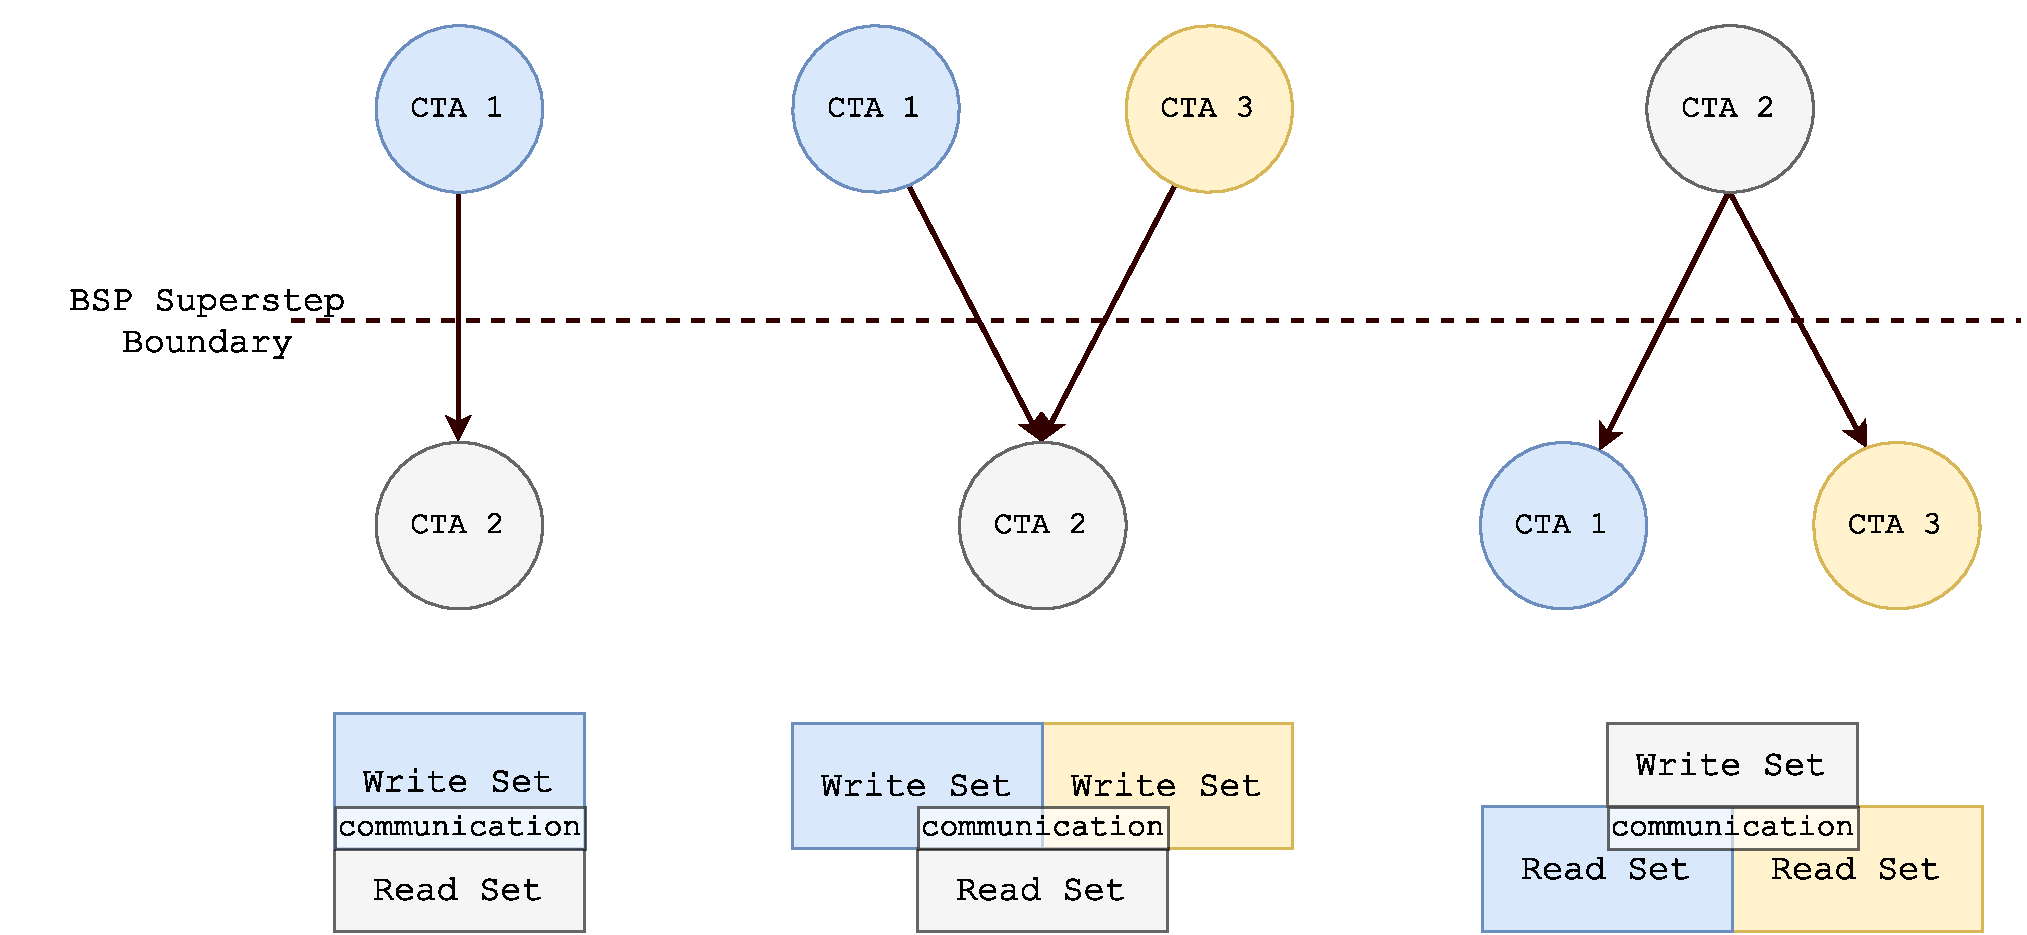
\includegraphics[width=\textwidth]{gpu-comm}
	\caption{Communication across a BSP superstep boundary, and how this corresponds to read and write sets 
	of sinks and sources. Edges are logical representations of communication, which is actually the overlap of write and read addresses in different BSP supersteps. Different colors represent different sink/source entities.}
	\label{gpu-comm}
\end{figure} 
To exemplify the definition above, figure \ref{gpu-comm} shows how communication between partners across a 
BSP superstep boundary translates to overlaps of write- and read-sets. The nodes above the superstep boundary are data sources, the nodes below sinks. The accumulated edge-weight is the size of the 
overlapping area in the write- and read-sets. 
This representation works for all levels of granularity in the hierarchy of the GPU execution model, from a single thread to an application using multiple kernels and streams.

\section{Analysis Space Exploration}

The analysis space for this work is multi-dimensional, created by the hierarchical execution model and BSP design.
The dimensions consist of:
\begin{itemize}
	\item Threads
	\item CTA
	\item Supersteps
	\item Different Kernels
\end{itemize}
At first it seems, these points may be a stepping of granularity, rather than different dimensions. The following four vectors describe interactions of dimensions during different analyses.
 \begin{align}
a &= \begin{bmatrix}
0 \\
0 \\
1\\
0
\end{bmatrix} &
b &= \begin{bmatrix}
0 \\
0 \\
0\\
1
\end{bmatrix} &
c &= \begin{bmatrix}
0 \\
1 \\
0\\
1
\end{bmatrix} &
d &= \begin{bmatrix}
0 \\
1 \\
1\\
0
\end{bmatrix}
\end{align}
Vector $(a)$ describes an anlysis that only takes kernel interactions into consideration, for example the communicated volumes across as BSP superstep boundary. Vetor $(b)$ describes how different kernels interact 
\subsection{Premises and Simplifications}

This work uses CTAs as the fundamental entities of communication source and sink. A kernel execution is a BSP superstep and is serialized with follow-up kernel iterations, or supersteps. Each stream is treated as
an individual BSP entity during the execution. Stream interactions can be recreated in the follow-up analysis.
\subsection{Collective Communication}
While MPI offers collective communication with clear definitions such as scatter, gather or multicast, the implicit memory communication of GPUs often can not be categorized as clearly. However the in- and out-degree of a communication node can give indications on tendencies towards a certain kind of collective.
For the sake of the analysis, each "collective" communication can be viewed as a set of point-to-point
communications, happening at the same time.  


\begin{itemize}
	\item BSP-Boundary oriented. What happens 'across' boundaries on the GPU. Ignore individual kernels for now
	\item ignoring programs not "well-written" (CTA interaction inside the kernel)
	\item How is communication realised in shared memory: bobbels to read/write sets
	\item On collectives: no hard collectives, rather tendencies toward collective behaviour
\end{itemize}